\title{Irregular seismic data reconstruction using a percentile-half-thresholding algorithm}

\author{Yangkang Chen\footnotemark[1], Keling Chen\footnotemark[2], Peidong Shi\footnotemark[3] and Yanyan Wang\footnotemark[3]}

\address{
\footnotemark[1]Bureau of Economic Geology, \\
Jackson School of Geosciences \\
The University of Texas at Austin \\
University Station, Box X \\
Austin, TX 78713-8924 \\
USA \\
%+1-5125478899 \\
ykchen@utexas.edu \\
%\ead{ykchen@utexas.edu}
\footnotemark[2]Department of Earth and Atmospheric Sciences \\
University of Houston, \\
Houston, TX, 77004\\
USA \\
kxc124930@gmail.com\\
\footnotemark[3]State Key Laboratory of Petroleum Resources and Prospecting \\
China University of Petroleum \\
Fuxue Road 18th\\
Beijing, China, 102200 \\
speedshi@126.com
%yanshan0425@126.com
}

%\maketitle

\lefthead{Chen et al.}
\righthead{percentile-half-thresholding algorithm}

% for multiple-revision
\DeclareRobustCommand{\dlo}[1]{\ifthenelse{\boolean{@revd}}{}{}}
\DeclareRobustCommand{\wen}[1]{%
  \ifthenelse{\boolean{@revd}}{\textcolor{black}{#1}}{#1}}

%\dlo means remove removing
%\wen means preserve

\begin{abstract}
%In this paper, we introduce a novel IST based iterative algorithm for reconstructing irregularly sampled seismic data. 
In this paper, a percentile-half-thresholding approach is proposed in the transformed domain thresholding process for iterative shrinkage thresholding (IST). The percentile-thresholding strategy is more convenient for implementing than the constant-value, linear-decreasing, or exponential-decreasing thresholding because it's data-driven. The novel half-thresholding strategy is inspired from the recent advancement in the researches on optimization using non-convex regularization. We summarize a general thresholding framework for IST and show that the only difference between half thresholding and the conventional soft or hard thresholding lays in the thresholding operator. Thus it's straightforward to insert the existing percentile-thresholding strategy to the half-thresholding iterative framework. We use both synthetic and field data examples to compare the performances using soft thresholding or half thresholding with constant threshold or percentile threshold. Synthetic and field data show consistent results that 
%half thresholding can achieve more precise reconstructed result than the conventional soft thresholding, and the percentile-thresholding approach can obtain better interpolated result than the constant-value thresholding. 
apart from the threshold-setting convenience, the percentile thresholding also has the possibility for improving the recovery performance. Compared with soft thresholding, half thresholding tends to have a more precise reconstructed result.
\end{abstract}

\section{Introduction}
Seismic data interpolation plays a fundamental role in seismic data processing, which provides the regularly sampled seismic data for the following jobs like 3D SRME and wave equation-based migrations \cite[]{shengxu2010}. There has been a number of effective methods to recover missing seismic traces, these methods can be generally divided into three types. The first kind is based on a convolution operator, which utilizes a prediction filter computed from the low-frequency parts to predict the high-frequency components \cite[]{spitz1991,porsani1999,wang2002}. However, the predictive filtering method can only be applied to regularly sampled seismic data \cite[]{mostafa2007}. The second type is a transformed domain method, which is based on a sparsity assumption and makes use of the theory of compressive sensing or compressive sampling (CS) \cite[]{candes20062,donoho2006,mallat2009,herrmann2010} to achieve a successful recovery using highly incomplete available data \cite[]{sacchi1998,wang2003,zwartjes20071,zwartjes20072,pengliang2012,pengliang2013}. \cite{mostafa2007} proposed a multistep autoregressive strategy which combines the first two types of methods to reconstruct irregular seismic data. The third type is based on the integral of continuation operators. This integral is performed based on the traveltime calculation from a velocity model, thus it depends on the known velocity model, which also becomes its limitation \cite[]{canning1996,bleistein2000,stolt2002,fomel2003}.

A recently very popular way for interpolating irregularly sampled seismic data is by using iterative thresholding, such as projection onto convex sets (POCS) and iterative shrinkage thresholding (IST), mainly because of their simple formulations and convenient implementations. Different thresholding approaches will lead to different performances for interpolation. 
%One simple way is constant-value thresholding. Other more efficient ways includes the linear-decreasing thresholding \cite[]{abma2006}, exponential decreasing \cite[]{jianjun2010}. 
Because of the advancement of the non-convex optimization algorithms, a half-thresholding algorithm has been proposed both in signal-processing and exploration geophysics communities \cite[]{pengliang20131,zongben2012}. In this paper, we summarize a general thresholding framework for IST algorithm. The only difference among soft, hard, and half thresholding lays in the thresholding operator. Thus, a percentile thresholding strategy, which is particularly useful in practice, can be straightforwardly applied to the case of half thresholding. We use both synthetic and field data examples to demonstrate the performance of our proposed percentile-half-thresholding algorithm, compared with other three existing approaches.


\section{Theory}
\subsection{Seismic interpolation}
The basic target of seismic interpolation is to solve the following equation:
\begin{equation}
\label{eq:int1}
\mathbf{d}_{obs}=\mathbf{Md},
\end{equation}
where $\mathbf{d}_{obs}$ is the observed data which is regularly or irregularly sampled, $\mathbf{d}$ is the unknown data we want to reconstruct and $\mathbf{M}$ is the sampling matrix. The sampling operator has a diagonal structure, which is composed by zero and identity matrix:
\begin{equation}
\label{eq:mask}
\mathbf{M} = \left[\begin{array}{cccccccc} 
\mathbf{I} & 	       & 	  & 	     &		 &	\\
	   &\mathbf{O} & 	  &	     &		 &	\\
	   &           &\mathbf{I}&	     &		 &	\\
	   &  	       &          &\mathbf{I}&	         & 	\\
	   &	       &	  &	     &\mathbf{\ddots} & \\
	   &	       &	  &	     &		 & \mathbf{I} 
\end{array}\right].
\end{equation}
Each $\mathbf{I}$ in equation \ref{eq:mask} corresponds to sampling a trace, and each $\mathbf{O}$ corresponds to missing a trace.

As equation \ref{eq:int1} is under-determined, additional constraint is required in order to solve the equation. By applying a regularization term, we get a least-squares minimization solution for solving equation \ref{eq:int1}:
\begin{equation}
\label{eq:int2}
\hat{\mathbf{d}}=\arg\min_{\mathbf{d}}\Arrowvert \mathbf{d}_{obs}-\mathbf{Md}\Arrowvert_2^2+\mathbf{R}(\mathbf{d}),
\end{equation}
where $\mathbf{R}$ is a regularization operator and $\Arrowvert\cdot\Arrowvert_2^2$ denotes the square of $L_2$ norm.

\subsection{Iterative shrinkage thresholding}
In order to reconstruct the missing traces in the seismic data, one can use a sparsity-promoting transform to precondition $\mathbf{d}$ in equation \ref{eq:int1}, that is:
\begin{equation}
\label{eq:precondition}
\mathbf{d}=\mathbf{Ax},
\end{equation}
where $\mathbf{A}$ is a tight frame such that $\mathbf{x}=\mathbf{A}^{H}\mathbf{d}$ and $\mathbf{A}^{-1}=\mathbf{A}^{H}$, and $[\cdot]^H$ denotes adjoint. A common selection for $\mathbf{A}$ is the Fourier transform.
Inserting equation \ref{eq:precondition} into equation \ref{eq:int1}, and let $\mathbf{K}=\mathbf{MA}$, we obtain 
\begin{equation}
\label{eq:forw2}
\mathbf{d}_{obs} = \mathbf{Kx}.
\end{equation}
Correspondingly, equation \ref{eq:int2} turns to:
\begin{equation}
\label{eq:int3}
\hat{\mathbf{x}} = \arg\min_{\mathbf{x}} \Arrowvert \mathbf{d}_{obs}-\mathbf{Kx} \Arrowvert_2 + \mathbf{R}'(\mathbf{x})
\end{equation}
The well-known IST algorithm is used for solving equation \ref{eq:int3} with a sparsity constraint:
\begin{equation}
\label{eq:ist}
\mathbf{x}_{n+1} = \mathbf{T}_{\gamma(\tau,p)}[\mathbf{x}_n+\mathbf{K}^{H}(\mathbf{d}_{obs}-\mathbf{Kx}_n)].
\end{equation}
Here $\mathbf{T}_{\gamma(\tau,p)}$ corresponds to a thresholding operator performed element-wise with threshold $\gamma(\tau,p)$ \cite[]{pengliang20131}. When $p=1$, $\gamma(\tau,1)=\tau$, $\mathbf{R}'(\cdot)=\tau \Arrowvert \cdot \Arrowvert_1$, where $\tau$ is a regularization parameter which controls the weight between misfit and constraint in the minimization problem, $\mathbf{T}_{\gamma(\tau,1)}$ corresponds to a soft-thresholding operator:
\begin{equation}
\label{eq:soft}
\mathbf{T}_{\gamma(\tau,1)}[v(\mathbf{x})] = \left\{ \begin{array}{ll}
v(\mathbf{x})-\gamma \frac{v(\mathbf{x})}{|v(\mathbf{x})|} & \text{for}\quad  |v(\mathbf{x})| > \gamma(\tau,1)  \\
0			      & \text{for}\quad  |v(\mathbf{x})| \le \gamma(\tau,1)
\end{array}\right.,
\end{equation} 
where $v(\mathbf{x})$ denotes the amplitude of each position-coordinate vector $\mathbf{x}$.
 When $p=0$, $\gamma(\tau,0)=\sqrt{2\tau}$, $\mathbf{R}'(\cdot)=\tau \Arrowvert \cdot \Arrowvert_0$, $\mathbf{T}_{\gamma(\tau,0)}$ corresponds to a hard\wen{-}thresholding operator:
\begin{equation}
\label{eq:hard}
\mathbf{T}_{\gamma(\tau,0)}[v(\mathbf{x})] = \left\{ \begin{array}{ll}
v(\mathbf{x}) 	 & \text{for}\quad  |v(\mathbf{x})| > \gamma(\tau,0)  \\
0			      & \text{for}\quad  |v(\mathbf{x})| \le \gamma(\tau,0)
\end{array}\right.,
\end{equation}
\subsection{Percentile half thresholding}
Recent research suggests that it's possible to reconstruct the seismic data using non-convex $L_p$-norm minimization, $0< p <1$. Particularly, iterative half thresholding has been developed both in signal processing and exploration geophysics communities \cite[]{zongben2012,pengliang20131}. The difference between half thresholding and the conventional soft thresholding is just the thresholding operator. When $p=1/2$, $\gamma(\tau,1/2)=\frac{3}{2}\tau^{2/3}$, $\mathbf{R}'(\cdot)=\tau \Arrowvert \cdot \Arrowvert_{1/2}^{1/2}$, $\mathbf{T}_{\gamma(\tau,1/2)}$ becomes a half-thresholding operator:
\begin{align}
\label{eq:half}
&\mathbf{T}_{\gamma(\tau,1/2)}[v(\mathbf{x})] = \\
&\left\{ \begin{array}{l}
\frac{2}{3}v(\mathbf{x})\left(1+\cos(\frac{2}{3}\pi - \frac{2}{3} \arccos(\frac{\tau}{8}(\frac{|v(\mathbf{x})|}{3})^{-\frac{3}{2}}))\right) \\
\quad\quad\quad  \text{for}\quad  |v(\mathbf{x})| > \gamma(\tau,1/2)  \\
0	\\
	\quad\quad\quad    \text{for}\quad  |v(\mathbf{x})| \le \gamma(\tau,1/2) \\
 %\quad &
\end{array}\right..
\end{align} 
The threshold $\gamma(\tau,p)$ can be constant, linear-decreasing \cite[]{abma2006} and exponential-decreasing \cite[]{jianjun2010}. However, all of these defining criterion are based on a prior knowledge about the data and is often not easy to choose. Instead, a processing-convenient percentile-thresholding strategy can be selected to overcome this inconvenience \cite[]{dian2008}. $\gamma(\tau,p)$ is selected as the $k$th largest absolute value among all $N$ values in the transformed domain, where the predefined percentile threshold $pc=k/N$ such that \dlo{$\gamma(\tau,p) = pc * MAX(|v(\mathbf{x})|)$. Here, $MAX$ denotes the maximum value of the transformed domain.}\wen{$\gamma(\tau,p)=prctile(|v(\mathbf{x})|,pc)$. Here, $prctile$ returns percentile $pc$ of the values in $|v(\mathbf{x})|$.} 

\subsection{Signal-to-noise ratio}
In order to test the convergence performance, we use the widely used measurement\cite[]{hennenfent2006,guochang2009,sep}:
\begin{equation}
\label{eq:snr}
SNR=10\log_{10} \frac{\Arrowvert \mathbf{d} \Arrowvert_2^2}{\Arrowvert\mathbf{d}-\hat{\mathbf{d}}\Arrowvert_2^2},
\end{equation} 
where the unit for $SNR$ is $dB$, $\mathbf{d}$ and $\hat{\mathbf{d}}$ denote the true and estimated data, respectively. 

\section{Examples}
We use two synthetic examples and one field data set to compare the performance of the aforementioned percentile-half-thresholding approach with the conventional thresholding approaches. For simplicity, we only compare half thresholding with soft thresholding in two cases: percentile and constant-value threshold. 

%The two examples are shown in Figure \ref{fig:linear,linear-zero,sean,sean-zero}. Figures \ref{fig:linear} and \ref{fig:sean} show the original seismic sections. Figures \ref{fig:linear-zero} and \ref{fig:sean-zero} show the decimated sections with 30\% traces randomly removed. 
The first example is a synthetic example that is composed of four linear events, one of which crosses the other three events. The original data is shown in Figure \ref{fig:linear}. After randomly removing 30\% traces, we create the decimated section, as shown in Figure \ref{fig:linear-zero}. Figure \ref{fig:data2,data3,data5,data6,diff2,diff3,diff5,diff6,diff2_10,diff3_10,diff5_10,diff6_10} show the reconstruction results for the first synthetic example. From the result using percentile half thresholding (Figure \ref{fig:data6}) and constant-value half thresholding (Figure \ref{fig:data3}), and their corresponding estimation error sections (the difference between the true data and estimated data), we can observe that half thresholding nearly do a perfect job while the percentile thresholding strategy helps obtain a even better result. Both conventional constant-value and percentile soft-thresholding results seem to have significant estimation error.  We can also observe that the percentile soft thresholding outperforms the constant-value soft thresholding by obtaining slightly less estimation error.   \wen{In order to better compare the error sections using different approaches, we amplified the magnitude of each error section shown in Figures \ref{fig:diff2}, \ref{fig:diff3}, \ref{fig:diff5} and \ref{fig:diff6} by multiplying the magnitude by 10 times. The magnitude amplified error sections are shown in Figures \ref{fig:diff2_10}, \ref{fig:diff3_10}, \ref{fig:diff5_10} and \ref{fig:diff6_10}. It's much clearer that the percentile-half-thresholding strategy obtains a much better performance than any other approaches.} The diagrams shown in Figure \ref{fig:SNRs} further prove the observations in that the converged result for percentile half thresholding has the largest SNR, which is followed by constant-value half thresholding, and the constant-value soft thresholding obtains the smallest SNR.

The second example is a hyperbolic-events synthetic example. The original data and decimated data with 30 \% traces randomly removed traces are shown in Figure \ref{fig:hyper,hyper-zero}. We apply four different thresholding approaches as mentioned above to this example and get the reconstructed results and their corresponding reconstruction error sections, which are shown in Figure \ref{fig:hyper-data2,hyper-data3,hyper-data5,hyper-data6,hyper-diff2,hyper-diff3,hyper-diff5,hyper-diff6}. Similarly, the reconstructed result for the proposed percentile half thresholding (shown in Figure \ref{fig:hyper-data6}) obtains the best results, causing negligible reconstruction error (shown in Figure \ref{fig:hyper-diff6}). The constant-value \dlo{soft}\wen{half} thresholding also performs well because the error section (shown in Figure \ref{fig:hyper-data3}) contains small amount of coherent signals. The reconstruction results for soft thresholding using either percentile or constant-value strategy (shown in Figures \ref{fig:hyper-data2} and \ref{fig:hyper-data5} )are not pleasant. \dlo{Because they cause a significant energy loss in the error sections as shown in Figures \ref{fig:hyper-diff2} and \ref{fig:hyper-diff5}.} \wen{Because they still contain some zero or weak-amplitude traces and cause a significant energy loss in the error sections as shown in Figures \ref{fig:hyper-diff2} and \ref{fig:hyper-diff5}, which indicates a failure in interpolating the missing traces.} From the convergence diagram as shown in Figure \ref{fig:hyper-SNRs}, we can conclude that the half-thresholding approaches outperforms the conventional soft-thresholding approaches, while the percentile-thresholding strategy can helps obtain better results that the constant-value strategy.


The third example is a field marine data, which was investigated widely in the literature \cite[]{fomel2002pwd,liuyang2011rna}. We can obtain a similar conclusion as the previous two examples. However, from the reconstructed data and the estimation error sections, the conventional soft-thresholding (both constant-value and percentile) results (shown in Figures \ref{fig:sean-data2} and \ref{fig:sean-data5}) suffer from a heavy useful-energy loss as shown in Figures \ref{fig:sean-diff2} and \ref{fig:sean-diff5} \wen{and the reconstructed data as shown in Figures \ref{fig:sean-data2} and \ref{fig:sean-data5} still contain some obvious zero or weak-amplitude traces}, which is no longer acceptable. From the convergence diagrams shown in Figure \ref{fig:sean-SNRs}, the \wen{final} SNRs of conventional soft-thresholding approaches are \dlo{both less than 12 $dB$}\wen{lower than the half-thresholding approaches.}. \dlo{The half-thresholding algorithms get much higher SNRs compared with soft-thresholding algorithms. The proposed percentile-half-thresholding obtains the highest SNR: 20 $dB$.}\wen{Although the constant-value half thresholding can get slightly higher SNR than percentile half thresholding during the first several iterations, the percentile half thresholding converges to a higher final SNR than constant-value half thresholding.}

\section{Conclusions}
We have introduced a general thresholding framework for IST algorithm. The only difference between half thresholding and conventional soft or hard thresholding is owing to the thresholding operator, so the percentile-thresholding strategy can be easily inserted into the half-thresholding algorithm. We compared four different types of thresholding strategies by using two synthetic examples and one field data example. The results show that apart from the threshold-setting convenience, the percentile thresholding also has the possibility for improving the recovery performance. Compared with soft thresholding, half thresholding tends to have a more precise reconstructed result.

\section{Acknowledgments}
We would like to thank Pengliang Yang for help discussions during his visit in UT Austin. We also thank \new{Sanyi Yuan, Shan Qu, and} \old{three}\new{two} anonymous reviewers for their constructive suggestions, which helped improve this paper. We are grateful to developers of the Madagascar software package for providing corresponding codes for testing the algorithms and preparing the figures. 

\AtEndDocument{
\begin{figure}[htb!]
  \centering
  \subfloat[]{\includegraphics[width=0.23\textwidth,height=0.3500\textwidth]{linear/Fig/linear}
    \label{fig:linear}}
  \subfloat[]{\includegraphics[width=0.23\textwidth,height=0.3500\textwidth]{linear/Fig/linear-zero}
    \label{fig:linear-zero}}
	\caption{(a) Synthetic data (linear events). (b) Decimated synthetic data (created by randomly removing 30\% traces).}
   \label{fig:linear,linear-zero}
\end{figure}

\begin{figure}[htb!]
  \centering
  \subfloat[]{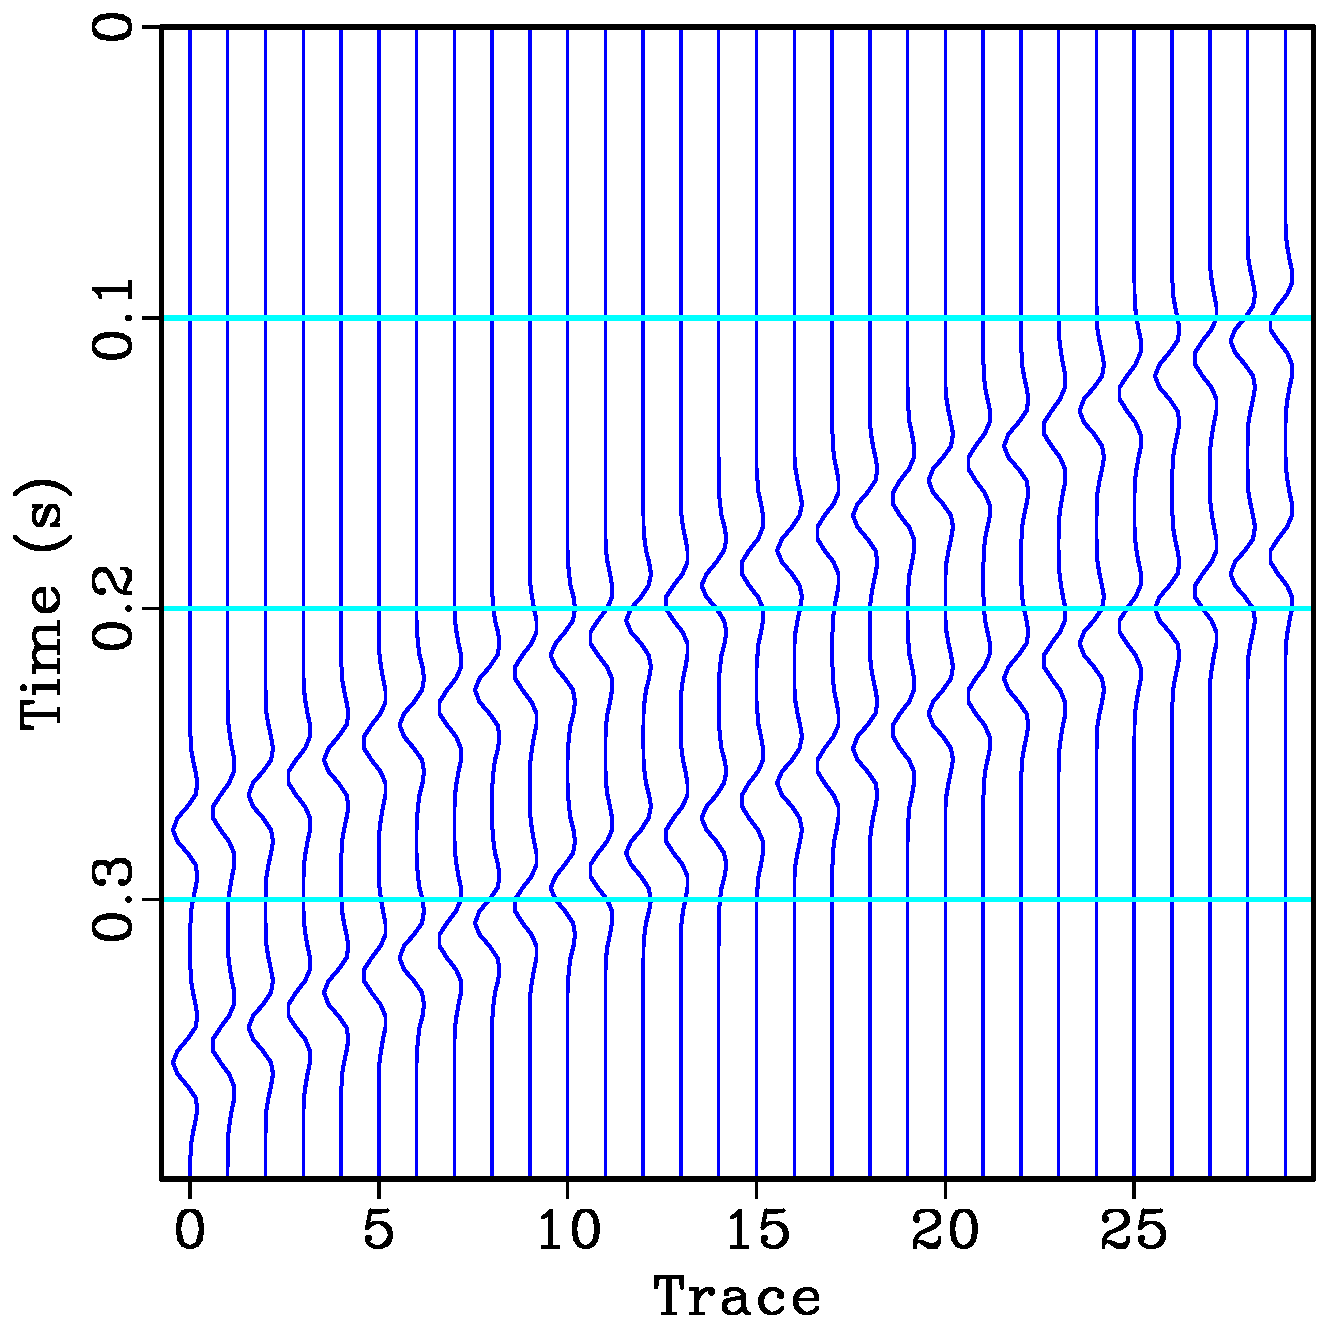
\includegraphics[width=0.23\textwidth,height=0.3100\textwidth]{linear/Fig/data2}
    \label{fig:data2}}
  \subfloat[]{\includegraphics[width=0.23\textwidth,height=0.3100\textwidth]{linear/Fig/data3}
    \label{fig:data3}}
  \subfloat[]{\includegraphics[width=0.23\textwidth,height=0.3100\textwidth]{linear/Fig/data5}
    \label{fig:data5}}  
  \subfloat[]{\includegraphics[width=0.23\textwidth,height=0.3100\textwidth]{linear/Fig/data6}
    \label{fig:data6}}      
  \subfloat[]{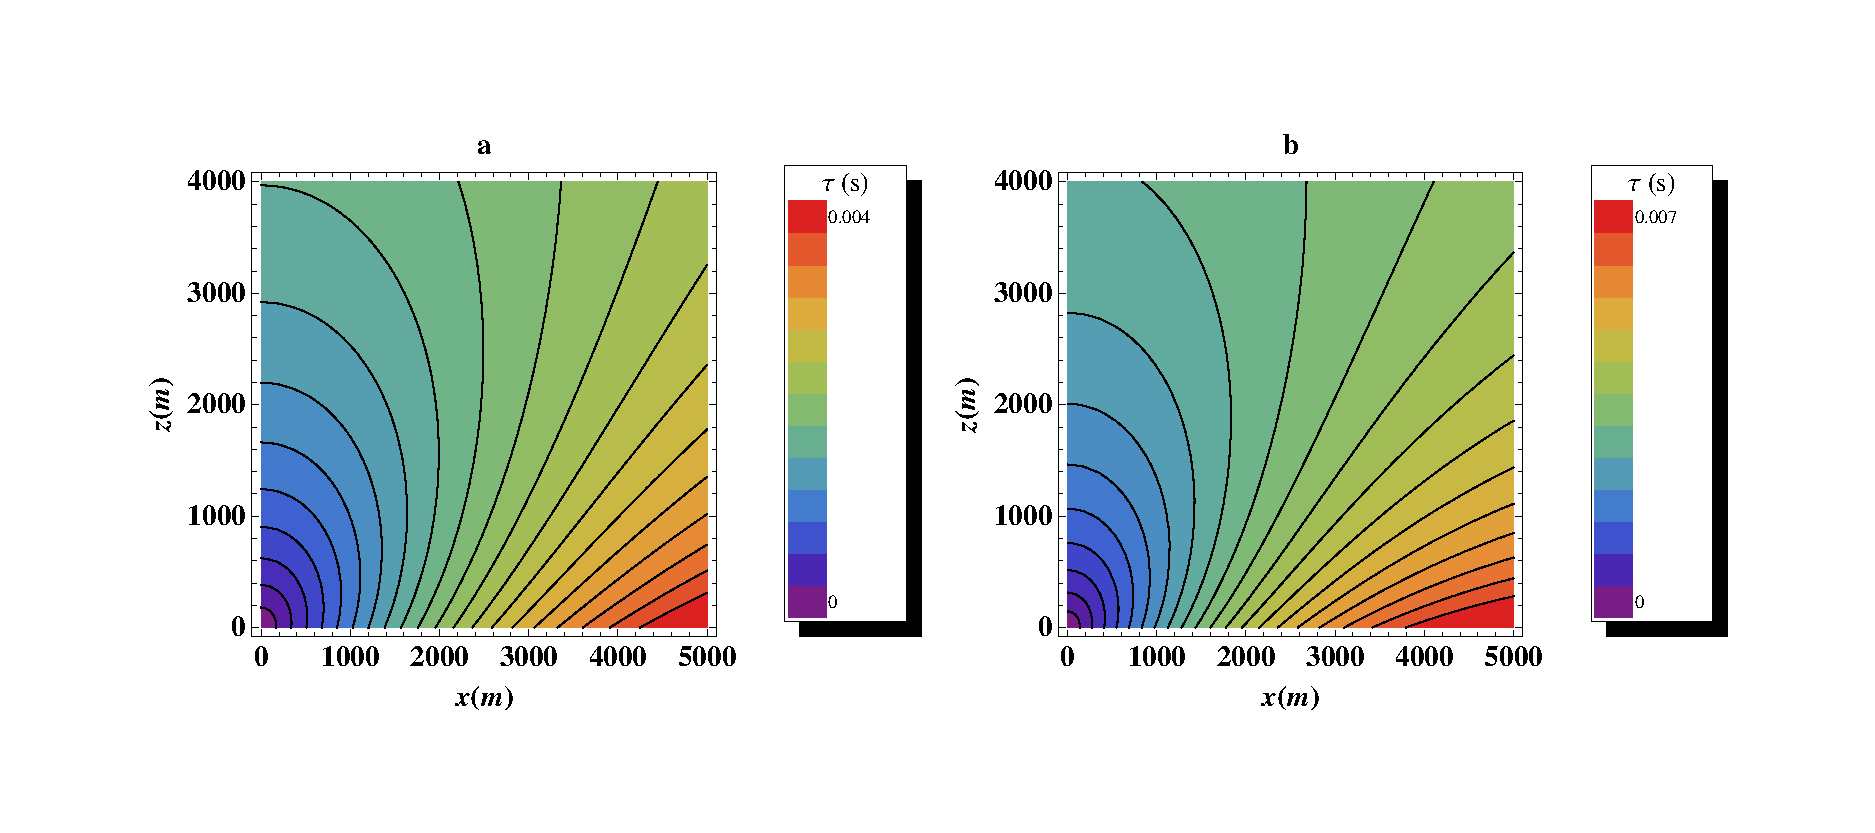
\includegraphics[width=0.23\textwidth,height=0.3100\textwidth]{linear/Fig/diff2}
    \label{fig:diff2}}
  \subfloat[]{\includegraphics[width=0.23\textwidth,height=0.3100\textwidth]{linear/Fig/diff3}
    \label{fig:diff3}}
  \subfloat[]{\includegraphics[width=0.23\textwidth,height=0.3100\textwidth]{linear/Fig/diff5}
    \label{fig:diff5}}
  \subfloat[]{\includegraphics[width=0.23\textwidth,height=0.3100\textwidth]{linear/Fig/diff6}
    \label{fig:diff6}}
  \subfloat[]{\includegraphics[width=0.23\textwidth,height=0.3100\textwidth]{linear/Fig/diff2_10}
    \label{fig:diff2_10}}    
  \subfloat[]{\includegraphics[width=0.23\textwidth,height=0.3100\textwidth]{linear/Fig/diff3_10}
    \label{fig:diff3_10}}
  \subfloat[]{\includegraphics[width=0.23\textwidth,height=0.3100\textwidth]{linear/Fig/diff5_10}
    \label{fig:diff5_10}}
  \subfloat[]{\includegraphics[width=0.23\textwidth,height=0.3100\textwidth]{linear/Fig/diff6_10}
    \label{fig:diff6_10}}    
	\caption{Reconstructed results for synthetic data (linear events). (a) Using constant-value soft thresholding. (b) Using constant-value half thresholding.  (c) Using percentile soft thresholding. (d) Using percentile half thresholding.  (e)-(h) Reconstruction error sections corresponding to (a)-(d), respectively.  (i)-(l) Amplitude amplified error sections by $\times 10$, corresponding to (e)-(h), respectively.}
   \label{fig:data2,data3,data5,data6,diff2,diff3,diff5,diff6,diff2_10,diff3_10,diff5_10,diff6_10}
\end{figure}

\begin{figure}[htb!]
  \centering
  \includegraphics[width=0.8\textwidth,height=0.6\textwidth]{linear/Fig/SNRs}

	\caption{Convergence diagrams for synthetic data (linear events). "p" corresponds to percentile half thresholding. "o" corresponds to constant-value half thresholding. "s" corresponds to percentile soft thresholding. "*" corresponds to constant-value soft thresholding. }
	    \label{fig:SNRs}
\end{figure}


\begin{figure}[htb!]
  \centering
  \subfloat[]{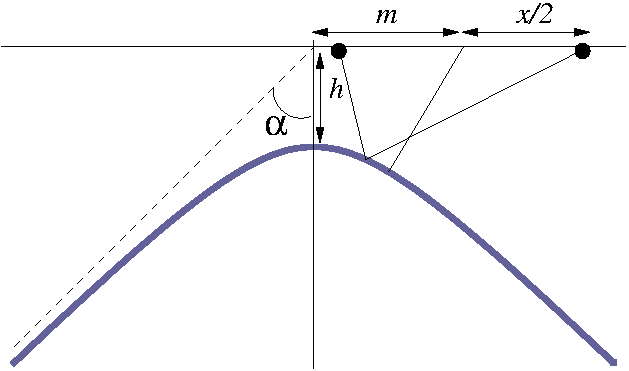
\includegraphics[width=0.23\textwidth,height=0.3500\textwidth]{hyper/Fig/hyper}
    \label{fig:hyper}}
  \subfloat[]{\includegraphics[width=0.23\textwidth,height=0.3500\textwidth]{hyper/Fig/hyper-zero}
    \label{fig:hyper-zero}}
	\caption{(a) Synthetic data (hyperbolic events). (b) Decimated synthetic data (created by randomly removing 30\% traces). }
   \label{fig:hyper,hyper-zero}
\end{figure}


\begin{figure}[htb!]
  \centering
   \subfloat[]{\includegraphics[width=0.23\textwidth,height=0.3500\textwidth]{hyper/Fig/hyper-data2}
    \label{fig:hyper-data2}}
  \subfloat[]{\includegraphics[width=0.23\textwidth,height=0.3500\textwidth]{hyper/Fig/hyper-data3}
    \label{fig:hyper-data3}}
  \subfloat[]{\includegraphics[width=0.23\textwidth,height=0.3500\textwidth]{hyper/Fig/hyper-data5}
    \label{fig:hyper-data5}}    
  \subfloat[]{\includegraphics[width=0.23\textwidth,height=0.3500\textwidth]{hyper/Fig/hyper-data6}
    \label{fig:hyper-data6}}    
  \subfloat[]{\includegraphics[width=0.23\textwidth,height=0.3500\textwidth]{hyper/Fig/hyper-diff2}
    \label{fig:hyper-diff2}}    
  \subfloat[]{\includegraphics[width=0.23\textwidth,height=0.3500\textwidth]{hyper/Fig/hyper-diff3}
    \label{fig:hyper-diff3}}
  \subfloat[]{\includegraphics[width=0.23\textwidth,height=0.3500\textwidth]{hyper/Fig/hyper-diff5}
    \label{fig:hyper-diff5}}
  \subfloat[]{\includegraphics[width=0.23\textwidth,height=0.3500\textwidth]{hyper/Fig/hyper-diff6}
    \label{fig:hyper-diff6}}
	\caption{Reconstructed results for synthetic data (hyperbolic events). (a) Using constant-value soft thresholding. (b) Using constant-value half thresholding.  (c) Using percentile soft thresholding. (d) Using percentile half thresholding.  (e)-(h) Reconstruction error sections corresponding to (a)-(d), respectively.}
   \label{fig:hyper-data2,hyper-data3,hyper-data5,hyper-data6,hyper-diff2,hyper-diff3,hyper-diff5,hyper-diff6}
\end{figure}

\begin{figure}[htb!]
  \centering
  \includegraphics[width=0.8\textwidth,height=0.6\textwidth]{hyper/Fig/hyper-SNRs}

	\caption{Convergence diagrams for synthetic data (hyperbolic events). "p" corresponds to percentile half thresholding. "o" corresponds to constant-value half thresholding. "s" corresponds to percentile soft thresholding. "*" corresponds to constant-value soft thresholding. }
	    \label{fig:hyper-SNRs}
\end{figure}


\begin{figure}[htb!]
  \centering
  \subfloat[]{\includegraphics[width=0.23\textwidth,height=0.3500\textwidth]{sean/Fig/sean}
    \label{fig:sean}}
  \subfloat[]{\includegraphics[width=0.23\textwidth,height=0.3500\textwidth]{sean/Fig/sean-zero}
    \label{fig:sean-zero}}
	\caption{(a) Field data. (b) Decimated field data (created by randomly removing 30\% traces).}
   \label{fig:sean,sean-zero}
\end{figure}

\begin{figure}[htb!]
  \centering
  \subfloat[]{\includegraphics[width=0.23\textwidth,height=0.3500\textwidth]{sean/Fig/sean-data2}
    \label{fig:sean-data2}}
  \subfloat[]{\includegraphics[width=0.23\textwidth,height=0.3500\textwidth]{sean/Fig/sean-data3}
    \label{fig:sean-data3}}
  \subfloat[]{\includegraphics[width=0.23\textwidth,height=0.3500\textwidth]{sean/Fig/sean-data5}
    \label{fig:sean-data5}}
  \subfloat[]{\includegraphics[width=0.23\textwidth,height=0.3500\textwidth]{sean/Fig/sean-data6}
    \label{fig:sean-data6}}
  \subfloat[]{\includegraphics[width=0.23\textwidth,height=0.3500\textwidth]{sean/Fig/sean-diff2}
    \label{fig:sean-diff2}}
  \subfloat[]{\includegraphics[width=0.23\textwidth,height=0.3500\textwidth]{sean/Fig/sean-diff3}
    \label{fig:sean-diff3}}
  \subfloat[]{\includegraphics[width=0.23\textwidth,height=0.3500\textwidth]{sean/Fig/sean-diff5}
    \label{fig:sean-diff5}}
  \subfloat[]{\includegraphics[width=0.23\textwidth,height=0.3500\textwidth]{sean/Fig/sean-diff6}
    \label{fig:sean-diff6}}
	\caption{Reconstructed results for field data.  (a) Using constant-value soft thresholding. (b) Using constant-value half thresholding.  (c) Using percentile soft thresholding. (d) Using percentile half thresholding.  (e)-(h) Reconstruction error sections corresponding to (a)-(d), respectively.}
   \label{fig:sean-data2,sean-data3,sean-data5,sean-data6,sean-diff2,sean-diff3,sean-diff5,sean-diff6}
\end{figure}

\begin{figure}[htb!]
  \centering
  \includegraphics[width=0.8\textwidth,height=0.6\textwidth]{sean/Fig/sean-SNRs}
	\caption{Convergence diagrams for field data. "p" corresponds to percentile half thresholding. "o" corresponds to constant-value half thresholding. "s" corresponds to percentile soft thresholding. "*" corresponds to constant-value soft thresholding. }
	    \label{fig:sean-SNRs}
\end{figure}
}



\bibliographystyle{seg}
\bibliography{halfthr}
\newpage
\listoffigures
\newpage









